\documentclass[tikz]{standalone}
\begin{document}
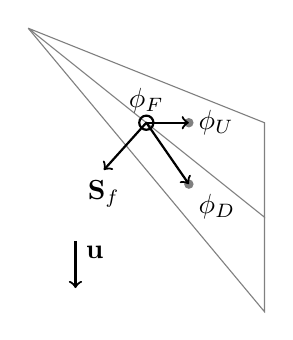
\begin{tikzpicture}[
  scale=0.6, 
  cpnt/.style={fill=gray}
]
\draw [thick, ->] (1,5.5) -- (1,4.5) node [near start, anchor=west] {$\mathbf{u}$};

\draw [gray] (0,10) -- (5,8) -- (5,6) -- (0,10);
\draw [gray] (0,10) -- (5,4) -- (5,6);

\draw [thick] (2.5,8) circle [radius=0.15] node [anchor=south] {$\phi_F$};
\path [cpnt] (3.4,8) circle [radius=0.1] node [anchor=west] {$\phi_U$};
\path [cpnt] (3.4,6.7) circle [radius=0.1] node [anchor=north west] {$\phi_D$};

\draw [thick,->,line cap=round] (2.5,8) -- (1.6,7) node [at end, anchor=north] {$\mathbf{S}_f$};
\draw [thick,->,line cap=round] (2.5,8) -- (3.4,8);
\draw [thick,->,line cap=round] (2.5,8) -- (3.4,6.7);
\end{tikzpicture}
\end{document}
